The goal of our work is to analyze a web API statically and from this analysis, 
without deploying or running the web API, 
to accurately estimate an upper bound on its response time. With such a prediction,
developers and cloud administrators can provide performance SLAs to the clients (human or 
programmatic) of web APIs, to help them reason about 
the performance implications of their use -- something that is not possible today.
For general purpose applications, such worst-case execution time analysis has been shown
by numerous researchers to be challenging to achieve for all but 
simple programs or specific application domains.

To overcome these challenges, we take inspiration from the latter and exploit 
the application domain of PaaS-hosted web APIs to achieve our goal.  
In this paper, we focus on the popular Google App Engine (GAE) public PaaS 
and AppScale private PaaS, which support the same applications, 
development and deployment model, and platform services.

The first characteristic of PaaS systems
that we exploit to faciliate our analysis 
is their predefined programming interfaces 
through which they export various platform services. 
Herein we refer to these programming interfaces as the cloud software development 
kit or the \textit{cloud SDK}. We refer to the individual member interfaces of the cloud SDK
as \textit{cloud SDK interfaces}, and to their constituent operations 
as \textit{cloud SDK operations}.  These interfaces export scalable
functionality that is commonly used for implementation of web APIs:  
key-value datastores, databases,
data caching, task and user management, security and authentication, etc.
The App Engine and AppScale cloud SDK is detailed 
in \url{https://cloud.google.com/appengine/docs/java/javadoc/}. 

%App Engine, for example, provides several cloud SDKs; one for each
%programming language supported (Java, Python, Go etc). Each SDK consists of
%several cloud SDK interfaces. Table~\ref{tab:gae_cloud_sdk} lists some of them.
%Each individual interface is comprised of several cloud SDK operations. For instance, the 
%datastore interface of App Engine provides operations for saving an entity (a data object),
%deleting an entity, and querying the datastore to read one or more entities.

%\begin{table}[htdp]
%\caption{Google App Engine cloud SDK interfaces}
%\begin{center}
%\begin{tabular}{|c|p{5cm}|}
%\hline
%Cloud SDK Interface & Functionality \\ \hline
%datastore & Reading and writing data to a highly scalable database with some transaction support. \\ \hline
%memcache & In-memory caching of data for faster access.\\ \hline
%users & User session management (login and logout)\\ \hline
%blobstore & Reading and writing large chunks (blobs) of uninterpreted bytes.\\ \hline
%task queue & Scheduling periodic and background jobs.\\ \hline
%\end{tabular}
%\end{center}
%\label{tab:gae_cloud_sdk}
%\end{table}

\begin{figure}
\centering
%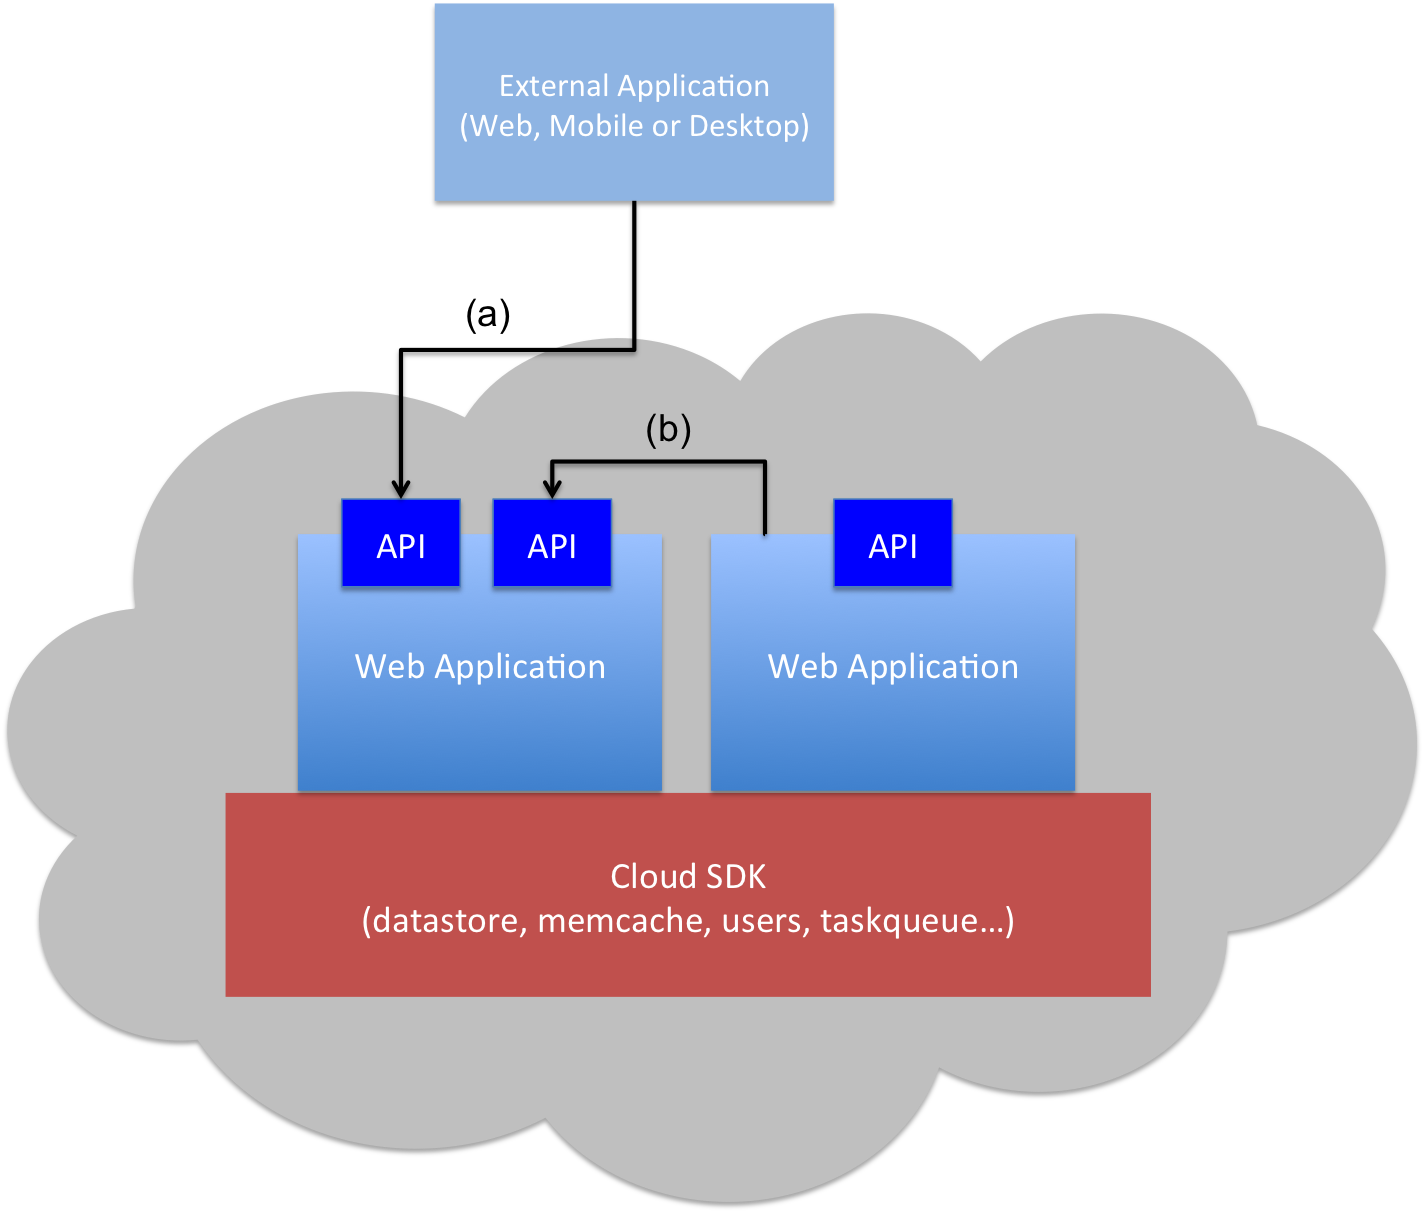
\includegraphics[scale=0.35]{cloud_app_model}
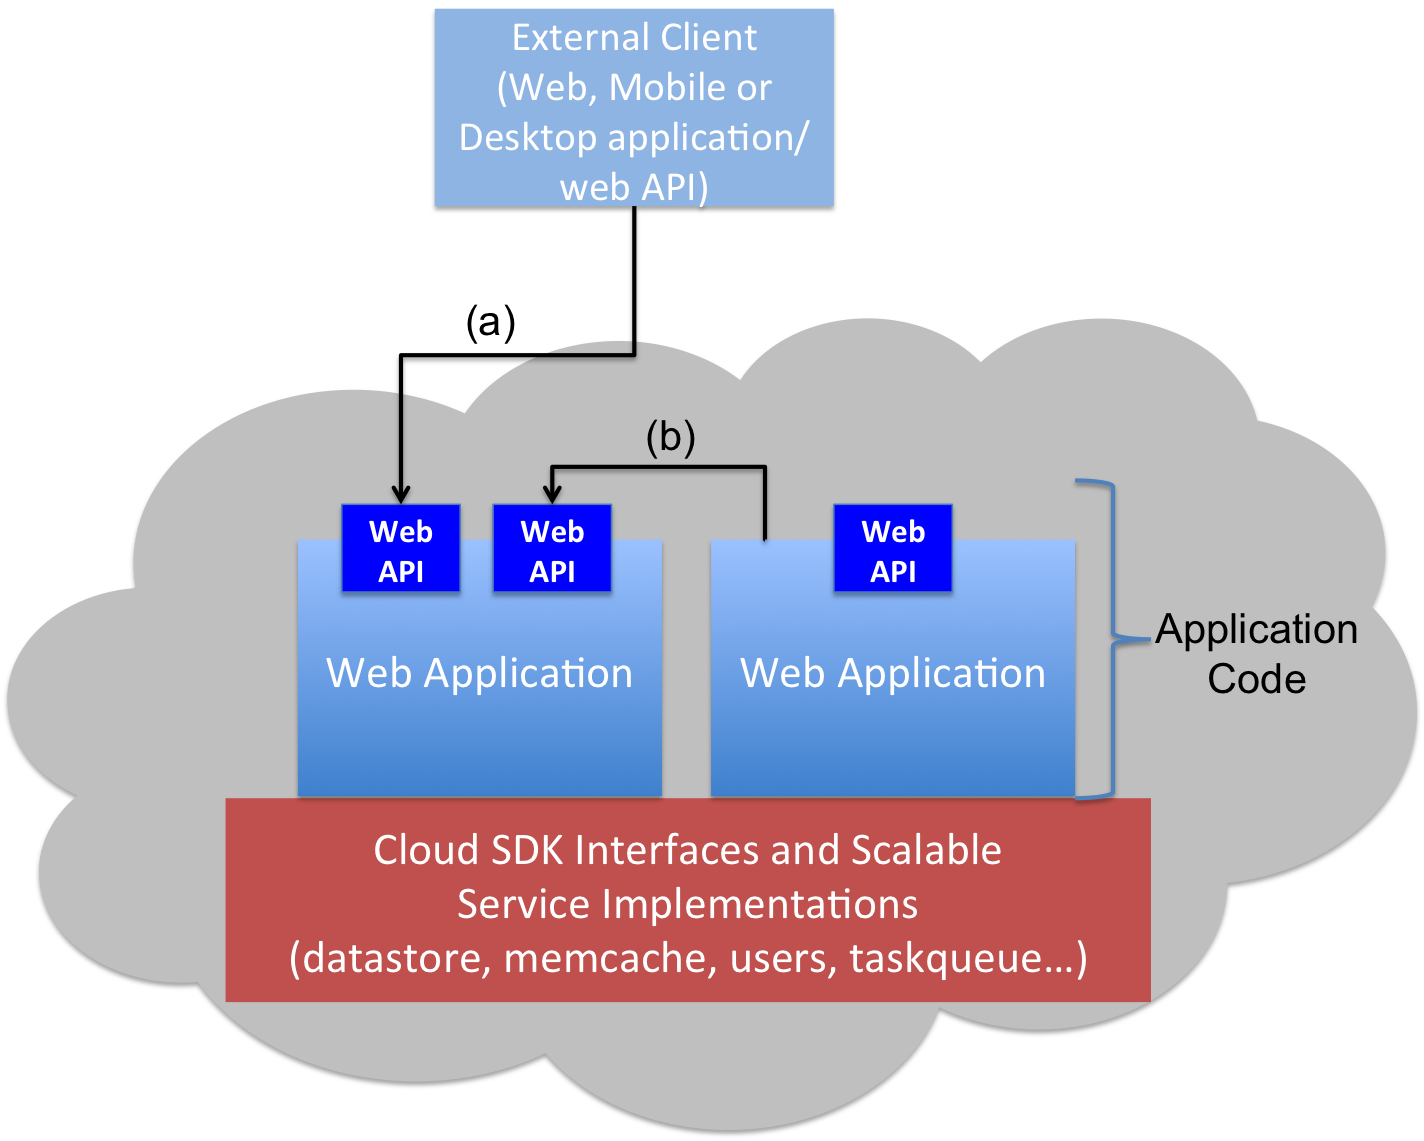
\includegraphics[scale=0.35]{sdk}
\caption{PaaS-hosted Web APIs: (a) An external client making requests
to the API;
(b) A Paas-hosted web API invoking another in the same cloud.
\label{fig:cloud_app_model}
}
\vspace{-0.1in}
\end{figure}

Figure~\ref{fig:cloud_app_model} illustrates the PaaS development and deployment model.
Developers implement their applications using a combination of operations
from the cloud SDK and their own code.  The service implementations for the 
cloud SDK are highly scalable, highly available (have SLAs associated with them),
and automatically managed by the platform. Developers then
upload their applications to the cloud.
Once deployed, the applications and any web APIs exported by them can be accessed 
via HTTP/s requests by external or co-located clients.

Typically, PaaS-hosted web APIs perform one or more
cloud SDK calls.  The reason for this is two-fold.  First, 
cloud SDKs provide web APIs with much of the functionality that they require.
Second, PaaS clouds ``sandbox'' web APIs to enforce quotas, to enable billing,
and to restrict certain functionality
that can lead to security holes, platform instability, or scaling issues~\cite{gae-sandbox}.
For example, GAE and AppScale cloud platforms restrict the application code
from accessing the local file system, accessing shared memory, using certain libraries,
and arbitrarily spawning threads.

In particular, the only way for a web API to execute is in response
to an HTTP/S request or as a background task.  Therefore, execution of
all web API operations start and end at well defined program points, and
we are able to infer this structure from common software patterns.  Second,
concurrency is restricted by capping the number of threads
and requiring that a thread cannot outlive the request
that creates it.  Third, PaaS clouds enforce quotas and limits on service
(cloud SDK) use~\cite{azure-limits,gae-limits,gae-sandbox}.
App Engine for example, requires that all web API requests complete in 60 seconds.
Otherwise they are terminated by the platform. 
Such enforcement places a strict upper bound on the
execution of a web API operation.
